\chapter{Hệ thống nhúng và phần mềm nhúng}

%========== System ======================}
    \section{Hệ thống nhúng}

        \subsection{Định nghĩa}
Hệ thống nhúng(embedded system) là một thuật ngữ để chỉ một hệ thống có khả năng tự trị được nhúng vào trong một môi trường hay một hệ thống mẹ. Đó là  các hệ thống tích hợp cả phần cứng và phần mềm phục vụ các bài toán chuyên dụng trong nhiều lĩnh vực công nghiệp, tự động hóa điều khiển, quan trắc và truyền tin...Đặc điểm của các hệ thống nhúng là hoạt động ổn định và có tính năng tự động hóa cao.

Hệ thống nhúng thường được thiết kế để thực hiện một chức năng chuyên dụng, thường nó có khả năng tự hành và được thiết kế tích hợp vào một hệ thống lớn hơn để thực hiện một chức năng nào đó. Khác với các máy tính đa chức năng, một hệ thống nhúng chỉ thực hiện một hoặc một vài chức năng nhất định, thường đi kèm với những yêu cầu cụ thể và bao gồm một số thiết bị máy móc và phần cứng chuyên dụng mà ta không tìm thấy trong một máy tính đa chức năng nói chung.

Vì hệ thống chỉ được xây dựng cho một số nhiệm vụ nhất định nên cá nhà thiết kế có thể tối ưu hóa nó nhằm giảm thiểu kích thước và chi phí sản xuất. Các hệ thống nhúng thường được sản xuất hàng loạt với số lượng lớn. Hệ thống nhúng rất đa dạng và phong phú về chủng loại. Đó có thể là những thiết bị cầm tay nhỏ gọn như đồng hồ kĩ thuật số, máy chơi nhạc MP3 hoặc những sản phẩm lớn như cột đèn giao thông, bộ kiểm soát trong nhà máy... Xét về độ phức tạp, hệ thống nhúng có thể rất đơn giản với một vi điều khiển hoặc rất phức tạp với nhiều đơn vị, các thiết bị ngoại vi và mạng lưới được nằm gọn trong một lớp vỏ máy lớn. Các thiết bị như máy tính cầm tay cũng có một số đặc điểm tương tự với hệ thống nhúng.
Hệ thống nhúng bao gồm các thiết bị  phần cứng và phần mềm, hầu hết đều phải thỏa mãn yêu cầu hoạt động theo thời gian thực( real- time). Tùy theo tính chất và yêu cầu, mức độ đáp ứng của hệ thống có thẻ rất nhanh hoặc có thể chấp nhận một mức độ chậm chễ nhất định.

        \subsection{Độ tin cậy của hệ thống nhúng}
Các hệ thống nhúng thường nằm trong các cỗ máy được kì vọng là sẽ chạy hàng năm trời liên tục mà không gặp lỗi hoặc có thể khôi phục khi gặp lỗi. Vì thế các phần mềm và hệ thống nhúng được phát triển và kiểm thử một cách cẩn thận hơn là phần mềm cho máy tính cá nhân.

Ngoài ra, các thiết bị rời không đáng tin cậy như ổ đĩa, công tắc hoặc nút bấm thường được hạn chế sử dụng.

Một số vấn đề cụ thể về độ tin cậy như:
            \begin{itemize}
                \item Hệ thống không thể ngừng để sửa chữa một cách an toàn như  các hệ thống không gian, hệ thống dây cáp dưới biển, các đèn hiệu dẫn đường...Giải pháp đưa ra là  chuyển sang sử dụng các hệ thống con dự trữ hoặc các phần mềm cung cấp một phần chức năng.
                \item Hệ thống phải được chạy liên tục vì tính an toàn, ví dụ như các thiết bị dẫn đường máy bay, thiết bị kiểm soát độ an toàn trong các nhà máy hóa chất,… Giải pháp đưa ra là lựa chọn backup hệ thống.
                \item Nếu hệ thống ngừng hoạt động sẽ gây tổn thất rất nhiều tiền của ví dụ như các dịch vụ buôn bán tự động, hệ thống chuyển tiền, hệ thống kiểm soát trong các nhà máy...
            \end{itemize}

%================= Software ==================================
    \section{Phần mềm nhúng}

Là phần mềm trong các hệ thống nhúng. Phần mềm nhúng có thể là những chương trình đơn giản chạy trực tiếp trên nền phần cứng hoặc là những chương trình, ứng dụng chạy trên nền một hệ điều hành nhúng. Phần mềm nhúng thường chạy với số tài nguyên phần cứng hạn chế: không có bàn phím, màn hình hoặc có nhưng với kích thước nhỏ, bộ nhớ hạn chế.

Phần mềm nhúng thường được lập trình trên máy tính cá nhân của lập trình viên, được biên dịch với một trình biên dịch và một môi trường phát triển, máy tính dùng để lập trình được gọi là host. Sau đó chương trình được nạp lên thiết bị và chạy, thiết bị mà chương trình được nạp lên gọi la target.Với mỗi target khác nhau sẽ có cấu trúc vi điểu khiển khác nhau, và sử dụng hệ điều hành nhúng khác nhau, do vậy tùy từng loại sẽ có các cách thức lập trình tương ứng.

    
        
        \begin{figure}[H]
            \centering
            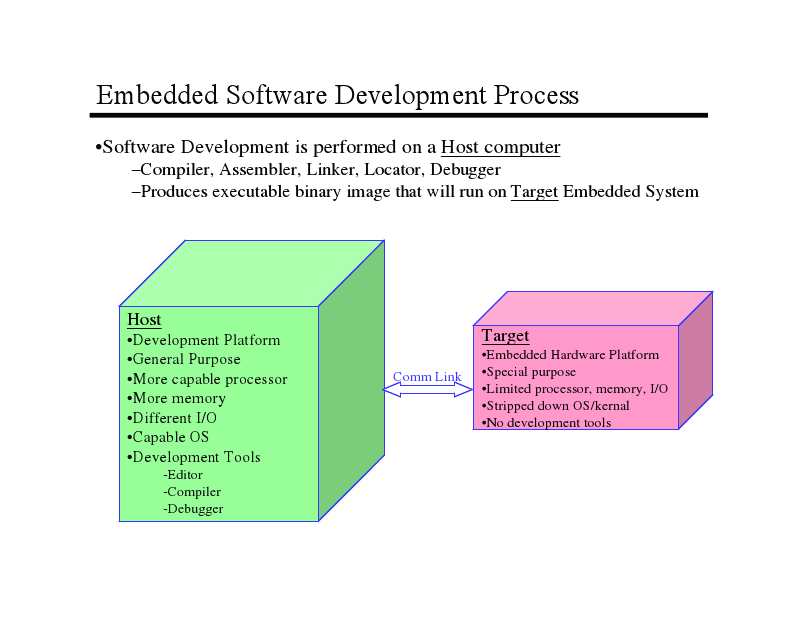
\includegraphics[scale=0.6]{hosttarget}
            \rule{35em}{0.5pt}
            \caption{Host và target trong phát triển phần mềm nhúng}
            \label{fig:hosttarget}
        \end{figure}

    C là một trong những ngôn ngữ lập trình nhúng phổ biến nhất hiện nay. C có một số ưu điểm nổi bật tiêu biểu như khá nhỏ và dễ dàng cho việc học, các chương trình biên dịch C thường khá sẵn cho hầu hết các bộ xử lý đang sử dụng hiện nay, và có rất nhiều người đã biết và làm chủ được ngôn ngữ này. 

 So với phần mềm thông thường, phần mềm nhúng có những điểm khác biệt sau:
    
    \begin{itemize}
        \item Phần mềm và phần cứng được phát triển cùng một lúc,
        \item Máy tính dùng để phát triển phần mềm (host) thường xuyên khác với target,
        \item Phần cứng cho target thường xuyên không có sẵn cho đến gần kết thúc dự án,
        \item Thương không rõ một lỗi nào đó là lỗi phần cứng hay lỗi phần mềm,
        \item Lỗi phần cứng thường được “chữa” bằng phần mềm,
        \item Số tiền bỏ ra cho phát triển phần mềm gấp hàng trăm lần so với phần cứng, do đó phần mềm thường được yêu cầu làm những việc mà nó nên được thực hiện bởi phần cứng,
        \item Có thể có ràng buộc về thời gian thực, xử lý song song, và vấn đề an toàn,
        \item Không có giao diện người-máy truyền thống, vì vậy các hoạt động của máy tính được giấu khỏi người dùng
        \item Thường có các ràng buộc về tài nguyên (bộ nhớ) hay mức tiêu thụ năng lượng.
    \end{itemize}

Với những đặc điểm này, việc phát triển phần mềm nhúng trở nên khó khăn hơn.
